\documentclass[10pt,a4paper]{article}
\usepackage[margin=1.9cm]{geometry}
\usepackage[T1]{fontenc}
\usepackage{lmodern}
\usepackage{microtype}
\usepackage{booktabs}
\usepackage{tabularx}
\usepackage{enumitem}
\usepackage{xcolor}
\usepackage{float}
\usepackage{caption}
\usepackage{tikz}
\usetikzlibrary{positioning,arrows.meta,fit,backgrounds,shapes.geometric}
\usepackage[colorlinks=true,linkcolor=blue!50!black,urlcolor=blue!50!black]{hyperref}
\setlist{nosep,leftmargin=1.2em}
\setlength{\parskip}{3pt}
\setlength{\parindent}{0pt}
\setlength{\emergencystretch}{3em}
\newcommand{\code}[1]{\texttt{#1}}
% Everything marked PENDING is filled from results/ (generated from real runs) -- never by hand.
\newcommand{\pending}[1]{\par\noindent\colorbox{yellow!40}{\parbox{\dimexpr\linewidth-2\fboxsep}{\textbf{PENDING:} #1}}\par}
\newcommand{\pendingi}[1]{\textcolor{orange!70!black}{\textbf{[PENDING: #1]}}}

\title{AutoSE: an Agentic Issue-to-PR Workflow for TinyDB\\
\large Architecture, decisions and evidence}
\author{Akshith Kandagatla (2024111004) --- Automated Software Engineering, Assignment 3}
\date{November 2026}

\begin{document}
\maketitle
\vspace{-1.5em}
\begin{center}\small
Fork: \url{https://github.com/Ohshit-ak/tinydb} (upstream \code{msiemens/tinydb} @ \code{edff96a}) \quad
Submission repo: \url{https://github.com/Ohshit-ak/autose-a3}\\
Models: Gemini \code{gemini-3.5-flash} (workers), \code{gemini-3.6-flash} (reviewer) \quad Full ADRs: \code{architecture/decisions/}
\end{center}

%=====================================================================
\section{Architecture}

\paragraph{Shape.} There are five LLM agents, each a separate Gemini session with its own system
prompt and its own function tools: Analyst, Architect, Builder, Tester and Reviewer. Two
deterministic components do the work that needs no judgment: the \emph{Controller} (a state machine
that runs every stage check and decides every back-edge) and \emph{Release} (push + PR).

The workflow is split into GitHub Actions jobs \emph{by permission}:
\begin{itemize}
\item jobs that hold the model key (\code{agents}, \code{review}) have tokens that cannot write;
\item jobs that can write (\code{release}, \code{post-review}, \code{ci-status}) never run a model and
  never execute model-written code.
\end{itemize}

\begin{figure}[H]\centering
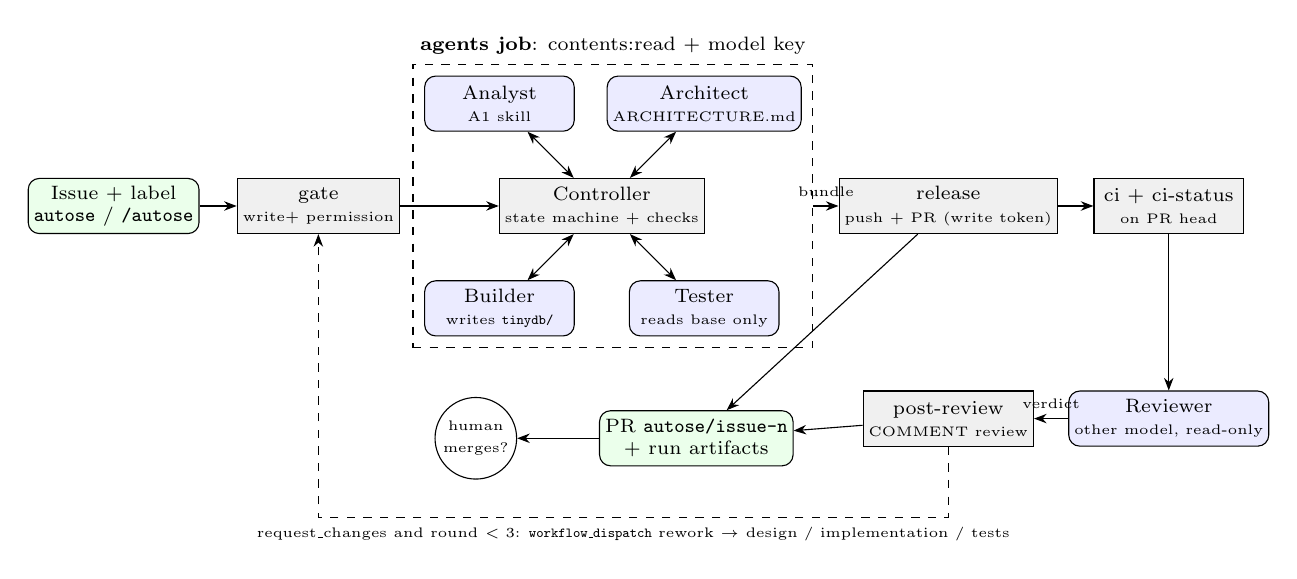
\begin{tikzpicture}[font=\scriptsize,
  ag/.style={draw, rounded corners, fill=blue!8, align=center, minimum height=7mm, minimum width=19mm, inner sep=2pt},
  det/.style={draw, fill=gray!12, align=center, minimum height=7mm, minimum width=19mm, inner sep=2pt},
  gh/.style={draw, fill=green!8, align=center, rounded corners=4pt, minimum height=7mm, inner sep=2pt},
  >={Stealth[length=1.6mm]}]
\node[gh]  (issue) at (0,0)    {Issue + label\\\code{autose} / \code{/autose}};
\node[det] (gate)  at (2.6,0)  {gate\\\tiny write+ permission};
\node[det, minimum width=24mm] (ctl) at (6.2,0) {Controller\\\tiny state machine + checks};
\node[ag]  (an)    at (4.9,1.3)  {Analyst\\\tiny A1 skill};
\node[ag]  (ar)    at (7.5,1.3)  {Architect\\\tiny ARCHITECTURE.md};
\node[ag]  (bu)    at (4.9,-1.3) {Builder\\\tiny writes \code{tinydb/}};
\node[ag]  (te)    at (7.5,-1.3) {Tester\\\tiny reads base only};
\begin{scope}[on background layer]
\node[draw, dashed, fit=(an)(ar)(bu)(te)(ctl), inner sep=4pt,
      label={[font=\scriptsize]above:\textbf{agents job}: contents:read + model key}] (aj) {};
\end{scope}
\node[det] (rel) at (10.6,0)   {release\\\tiny push + PR (write token)};
\node[det] (ci)  at (13.4,0)   {ci + ci-status\\\tiny on PR head};
\node[ag]  (rv)  at (13.4,-2.7) {Reviewer\\\tiny other model, read-only};
\node[det] (po)  at (10.6,-2.7) {post-review\\\tiny COMMENT review};
\node[gh]  (pr)  at (7.4,-2.95) {PR \code{autose/issue-n}\\+ run artifacts};
\node[draw, circle, inner sep=1pt, align=center] (hum) at (4.6,-2.95) {\tiny human\\\tiny merges?};
\draw[->] (issue) -- (gate); \draw[->] (gate) -- (ctl);
\foreach \a in {an,ar,bu,te} \draw[<->] (ctl) -- (\a);
\draw[->] (aj.east |- rel) -- node[above, font=\tiny]{bundle} (rel);
\draw[->] (rel) -- (ci); \draw[->] (ci) -- (rv); \draw[->] (rv) -- node[above,font=\tiny]{verdict} (po);
\draw[->] (rel) -- (pr); \draw[->] (po) -- (pr); \draw[->] (pr) -- (hum);
\draw[->, dashed] (po.south) -- ++(0,-0.9) -| node[pos=0.25, below, font=\tiny]{request\_changes and round $<3$: \code{workflow\_dispatch} rework $\to$ design / implementation / tests} (gate.south);
\end{tikzpicture}
\caption{Component view: agents, their tools/permissions and who calls whom (full version: \code{architecture/views/component.md}).}
\end{figure}

\begin{table}[H]\centering\scriptsize
\begin{tabularx}{\linewidth}{@{}l l l X l@{}}
\toprule
\# & Stage & Agent & Check (decided by the Controller, in code) & Artifact\\
\midrule
1 & Requirements & Analyst (A1 skill, unattended) & lint: \code{AC-n}, Given/When/Then, backticked observable, no vague words \textbf{and} LLM spec judge: every AC testable & \code{spec.md}\\
2 & Design & Architect (A2 ARCHITECTURE.md) & \code{Files to change} paths exist, functions found by AST (or NEW), every AC mapped, \code{Public interface} present & \code{design.md}\\
3 & Implementation & Builder & non-empty diff in allowlist (\code{tinydb/}, \code{docs/}); compileall + import (sandboxed) & \code{diff.patch}\\
4 & Testing & Tester + Controller & $\ge$1 \code{test\_ac<k>\_*} per AC; new tests and full suite pass; red-on-base recorded. Fail $\to$ stage 3 (3 attempts), 2nd fail $\to$ stage 2 once & \code{test\_report.md}\\
5 & Release & Release (code) & PR open (REST) and reusable \code{ci.yml} on the head sha succeeds (commit status on PR) & \code{pr.md} + link\\
6 & Review & Reviewer (separate job) & schema-valid verdict; approval needs a real \code{run\_tests} in the harness log; $\le$2 rework rounds & \code{review.md}\\
\bottomrule
\end{tabularx}
\caption{Stage map. A stage that cannot pass writes the reason into its artifact and the run stops.}
\end{table}

\textbf{Sequence of one real run.}\pending{sequence of the demo run (issue \#, run link, timings
from \code{state.json}, transitions), taken from \code{architecture/views/sequence.md} once the run exists.}

%=====================================================================
\section{Design decisions}

\begin{table}[H]\centering\scriptsize
\begin{tabularx}{\linewidth}{@{}l X X X X l@{}}
\toprule
ADR & Decision & Chosen & Main rejected option & Main reason & Status\\
\midrule
001 & Splitting the work & 5 role agents + deterministic Controller/Release & one agent for everything & separate contexts and tools; the writer never grades itself; no LLM holds the write token & Accepted\\
002 & Control flow & fixed state machine in one job; review rounds as self-dispatched runs & LLM planner/orchestrator & reproducible, bounded back-edges; no injected text can steer routing & Accepted\\
003 & Hand-offs & whole artifacts on need-to-know; structured feedback excerpts & shared transcript / LLM summaries & independence (Tester, Reviewer) and less injection surface; artifacts are small & Accepted\\
004 & State & workflow artifacts + one issue state comment; nothing on the PR branch & artifacts committed on the PR branch & the Reviewer sees the repo at head, so committed artifacts would leak reasoning & Accepted\\
005 & Tools & hand-written function tools, path jail, sandbox user; GitHub only in code jobs & GitHub MCP / generic bash for agents & least privilege that we can verify ourselves & Accepted\\
006 & Models & 2.5 Flash workers, 2.5 Pro reviewer & Pro everywhere & cost/rate limits vs.\ less correlated review errors & Superseded\\
011 & Models (new) & 3.5 Flash (low thinking) workers, 3.6 Flash reviewer & 4-hydrogen reviewer & 2.5 unavailable to new keys; latency is the binding limit & Accepted\\
007 & Checks & deterministic checks; LLM only judges AC testability; code decides & LLM judge per stage & judges can be argued with; checks must be reproducible & Accepted\\
008 & Reviewer independence & own job, token, model, inputs, adversarial evidence-based prompt & same job, new session & independence enforced by mechanisms, not convention & Accepted\\
009 & Safety \& failures & budgets at every level; capability containment over injection detection & LLM injection classifier & a hijacked agent can at most produce a bad diff & Accepted\\
010 & Triggers & label / \code{/autose} from write+ users; job-level queues & trigger on \code{issues: opened} & strangers cannot spend budget; no races on a branch & Accepted\\
\bottomrule
\end{tabularx}
\caption{ADR summary. \pendingi{status changes (Superseded / new ADRs) learned from real runs.}}
\end{table}

\paragraph{The three decisions that mattered most.}
\textbf{(1) Separating the model key from the write token (ADR-005/009).} Anyone can write an
issue, so we assume an agent \emph{will} sometimes follow injected text. The answer is capability,
not detection:
\begin{itemize}
\item the agents have no git, network or GitHub tools;
\item model-written code runs as a sandbox user with an empty environment;
\item the only jobs that can write never run a model.
\end{itemize}
Release re-checks the diff's paths deterministically, so even a hijacked Builder cannot change the
workflow. The cost is about 300 lines of our own tool harness.

\textbf{(2) Keeping state off the PR branch (ADR-004, enabling ADR-008).} This looked like a storage
detail but it decides reviewer independence. The Reviewer is allowed to see ``the repository at the
latest commit''. If spec, design and implementer notes were committed (the simplest durable store),
the Reviewer would read them. Workflow artifacts plus a state comment keep the run followable without
leaking reasoning.

\textbf{(3) Deterministic routing with a test oracle the Builder cannot touch (ADR-002/003/007).}
The Tester writes tests from the acceptance criteria while reading only the base commit. The Builder
cannot edit tests. The Controller, not an agent, decides when to retry or redesign. This makes
``tests pass'' mean something. The price is that a wrong test stops the run: a deliberate trade
of pass rate for honesty. \pendingi{evidence from runs: how often each back-edge fired.}

%=====================================================================
\section{Decision experiments}
Variants are defined in \code{experiment/variants.md} (fixed before any run).

\textbf{E1 --- ADR-008, independent vs.\ coupled reviewer, on 5 seeded PRs} (2 good, 3 with planted
defects, one carrying a prompt injection; labels fixed in advance).
\pending{table: per seeded PR, verdict A vs.\ B, planted defect named?, injection obeyed?, tokens.}

\textbf{E2 --- ADR-002/007, test-gated back-edges vs.\ single pass, on the 5 issues.}
\pending{table: per issue, stage-4 pass, hidden tests passed, tokens, wall time, A vs.\ B.}

\textbf{What we changed.} \pending{design changes and superseded ADRs that follow from E1/E2.}

%=====================================================================
\section{Results}
\pending{pass rate per stage (5 issues), hidden-test results per issue, what the reviewer caught and
where it was wrong, total tokens (sum of all \code{usage.jsonl}); all from \code{results/results.csv}.}

\paragraph{A finding from building the issue set.} Our first bug candidate (mutating a document returned
by \code{search()} corrupts the query cache) is pinned as \emph{intended} behaviour by an existing
upstream test (\code{test\_query\_cache\_documents\_are\_shared\_with\_cache}). Any fix must break that
test. Under our stage-4 rule (all existing tests pass, and agents may not edit existing tests) the run
would stop. That is correct for a bot, but it shows that the rule hands a legitimate class of change
(``the old behaviour was the bug'') to humans. We replaced the issue.

%=====================================================================
\section{Hindsight}
\pending{which decision we would change first, based on the runs.}

\section{Limitations and threats to validity}
\begin{itemize}
\item \textbf{Small sample.} 5 issues and 5 seeded PRs on one small, well-tested library. The pass rates
  have wide uncertainty and may not transfer to larger codebases.
\item \textbf{Hidden tests encode one reading of the vague issue} (issue 5: incomparable values do not
  match). An agent that chooses another reasonable reading (e.g.\ a clearer error) is counted as failing.
\item \textbf{Same author for issues, hidden tests and seeded defects.} The planted defects may be easier
  or harder than real ones, and the issues were written knowing the code.
\item \textbf{Non-determinism.} One run per (issue, variant) because of budget. LLM variance can change
  outcomes between identical runs.
\item \textbf{Model availability.} Results depend on the Gemini model versions available on the run date.
\end{itemize}

\end{document}
